\section{Rollback Netcode}

No contexto de videogames, alguns gêneros possuem problemas semelhantes aos que os ambientes musicais enfrentam. Aqueles que utilizam reações como uma das mecânicas de \textit{gameplay}, como luta e FPS (\textit{first-person shooter}), para implementar funcionalidades \textit{online}, necessitam que haja pouco atraso entre os \textit{inputs} dos jogadores.

Implementações de conexões \textit{online} em videogames são conhecidas popularmente como \textit{Netcode} - um termo não reconhecido oficialmente por fontes na Ciência da Computação, porém utilizado pelo público para classificar de forma geral as diferentes implementações. Há duas vertentes: (1) \textit{Delay-Based Netcode} e (2) \textit{Rollback Netcode} \cite{rollback}.

Em \textit{Delay-Based Netcode}, todos os \textit{inputs} dos transmissores são esperados antes que as ações correspondentes possam ser executadas \cite{rollback}. Essa implementação é a mais simples e garante a corretude dos dados transmitidos. No entanto, para conexões de alta latência, onde o tempo de transmissão via Internet seja maior que o tempo mínimo de ação localmente, os jogadores terão uma sensação de "lentidão".

Esse tempo mínimo de latência varia a cada jogo. Para oferecerem uma experiência fluida, de acordo com o tempo de reação à estímulos visuais, é esperado que não haja mais que 100 ms de atraso entre as ações dos jogadores \cite{pubnub}. Este limite, no entanto, é apenas uma estimativa - idealmente, a melhor implementação deve garantir que não haja diferença entre jogar \textit{online} ou localmente. Este limite dependerá de especificações de cada jogo, como FPS (\textit{frame-per-second}) e a latência natural causada pelo dispositivo de controle (\textit{input delay}). Desenvolvedores também podem adicionar um atraso artificial, para aumentar a janela de transmissão dos pacotes.

A implementação do \textit{Rollback Netcode}, por outro lado, aumenta a janela da espera dos pacotes propondo a previsão dos \textit{inputs} dos jogadores antes deles chegarem via Internet utilizando os dados já recebidos anteriormente (\figref{fig:rollback_diagram}). Caso as previsões sejam incorretas, o estado de jogo no momento em que a previsão foi realizado é retornado, portanto, o nome popular "\textit{rollback}" (reversão) \cite{rollback}.


\begin{figure}[htbp]
\centering
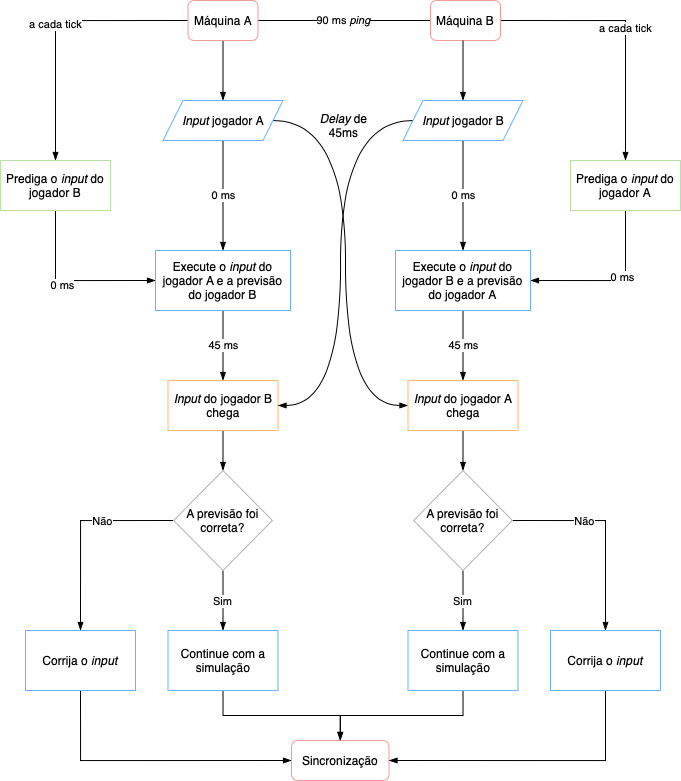
\includegraphics[width=1\textwidth]{images/rollback.png}
\caption{Diagrama demonstrando o processo de execução e sincronização dos \textit{inputs} de dois jogadores (com \textit{ping} de 90 ms entre eles) em um jogo \textit{online} utilizando \textit{Rollback Netcode} em um modelo \textit{peer-to-peer}. Tradução da imagem criada por GerardSN, CC BY-SA 4.0, https://commons.wikimedia.org/w/index.php?curid=97477279.}
\label{fig:rollback_diagram}
\end{figure}
